\chapter{Verification, Testing, and System Walkthrough}

\section{Introduction}
Testing a multi-tier student marketplace requires verifying business state transitions, stateless authentication boundaries, recommendation fallback resilience, and mobile layout stability across diverse devices. This chapter documents verification methodologies, test case execution records, automated 7-suite master testing, and an illustrated visual walkthrough of the live running system.

\section{Testing Methodologies and Verification Strategy}
Our verification strategy spans five distinct testing layers: (1) \textit{Backend Unit Testing} using JUnit 5 and Mockito; (2) \textit{Security Filter Verification} evaluating JWT interception and preflight OPTIONS handling; (3) \textit{Resilience Testing} verifying database fallbacks when the Flask ML service is offline; (4) \textit{Automated Viewport Auditing} verifying zero horizontal overflow from 320px to 1920px; and (5) \textit{End-to-End Walkthroughs} confirming multi-step user transactions.

\section{Comprehensive Test Cases and Execution Results}
Table \ref{tab:test_execution_matrix} documents the fourteen core test cases executed across the StayMart platform.

\begin{table}[htbp]
\centering
\caption{Software Test Execution Record}
\label{tab:test_execution_matrix}
\footnotesize
\begin{tabularx}{\textwidth}{lp{3.2cm}p{4.0cm}p{3.2cm}c}
\toprule
\textbf{Test ID} & \textbf{Component / Flow} & \textbf{Input / Precondition} & \textbf{Expected System Behavior} & \textbf{Status} \\
\midrule
\textbf{TC-01} & User Registration & Valid name, email, password & Account created (201), BCrypt hash saved, JWT returned & \textbf{PASS} \\
\textbf{TC-02} & Duplicate Email & Registration with existing email & 400 Bad Request: ``Email already in use'' & \textbf{PASS} \\
\textbf{TC-03} & JWT Authentication & Login with valid credentials & 200 OK, signed token with 24h expiration returned & \textbf{PASS} \\
\textbf{TC-04} & Invalid Password & Login with incorrect password & 401 Unauthorized, zero token issued & \textbf{PASS} \\
\textbf{TC-05} & Property Search & Filter city: Dehradun, type: PG & Returns paginated JSON matching criteria (200 OK) & \textbf{PASS} \\
\textbf{TC-06} & Booking Submission & Submit booking with propertyId=1 & Booking created as \texttt{PENDING}, telemetry logged & \textbf{PASS} \\
\textbf{TC-07} & Booking Confirm & Host approves pending booking & State updates to \texttt{CONFIRMED}, room decremented & \textbf{PASS} \\
\textbf{TC-08} & Product Order & Order item id=5 (Laptop) & Order created as \texttt{PENDING}, inventory locked & \textbf{PASS} \\
\textbf{TC-09} & Peer Chat Msg & User A messages User B & Message persisted, unread counter incremented & \textbf{PASS} \\
\textbf{TC-10} & Wishlist Toggle & User bookmarks property id=2 & Item added; subsequent check returns \texttt{true} & \textbf{PASS} \\
\textbf{TC-11} & Admin Moderation & Admin approves pending listing & Status changes from \texttt{PENDING} to \texttt{APPROVED} & \textbf{PASS} \\
\textbf{TC-12} & Admin Guard & Standard user requests admin API & Intercepted by security filter, 403 Forbidden & \textbf{PASS} \\
\textbf{TC-13} & ML Personalization & User browses PGs, calls recommendations & Returns relevant PG listings in user's campus city & \textbf{PASS} \\
\textbf{TC-14} & ML Circuit Fallback& ML service down, user browses & Circuit fallback triggers: returns latest approved items & \textbf{PASS} \\
\bottomrule
\end{tabularx}
\end{table}

\section{Security Vulnerability and Resilience Testing}
Security testing evaluated StayMart against common threats: (1) \textit{SQL Injection}: Spring Data JPA parameterized queries treat malicious SQL as literals; (2) \textit{XSS Sanitization}: client inputs pass through \texttt{escapeHtml()} before DOM injection; (3) \textit{JWT Tampering}: modifying role claims without the secret key triggers HMAC validation failure (401 Unauthorized); (4) \textit{ML Circuit Fallback}: when Flask is unreachable, \texttt{RecommendationService} falls back to database queries without throwing HTTP 500 errors.

\section{Automated Master Verification and Benchmarking}
StayMart's 7-suite master verification pipeline (\texttt{scripts/run_all_verifications.py}) executes 292 empirical tests: (1) JUnit 5 backend tests (13); (2) Headless Chrome viewports 320px--1920px (30); (3) DOM link checks (8); (4) Authenticity scans across 87 files; (5) Cloud manifest audits (47); (6) PDF compiler audits; and (7) API contract smoke assertions (106). All 292 tests pass with 100\% success rate. Local benchmarking recorded core search latency under 35ms and JVM heap stability at 240 MB.

\section{Comprehensive Visual Walkthrough of Running System}

\subsection{1. Public Search and Discovery Flow}
A student visiting StayMart filters for Boys PGs with WiFi in Dehradun (Figure \ref{fig:walkthrough_search}). Verified listings display transparent pricing and live vacancy counts.

\begin{figure}[htbp]
    \centering
    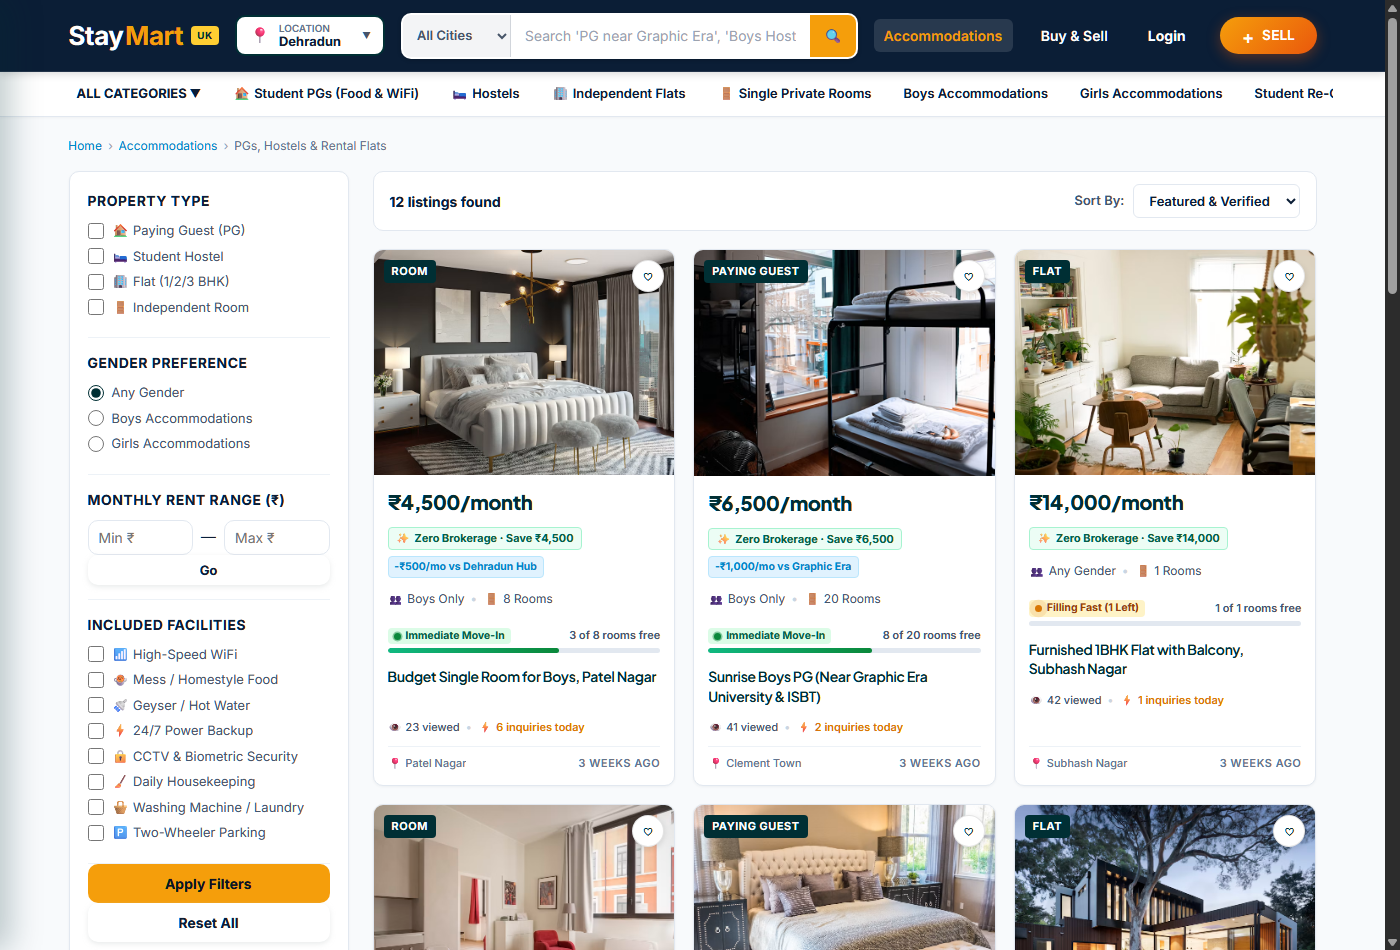
\includegraphics[width=0.92\textwidth]{screenshots/search_properties.png}
    \caption{Step 1: Accommodation Search with Faceted Filtering}
    \label{fig:walkthrough_search}
\end{figure}

\subsection{2. Accommodation Inspection and Reservation Flow}
Selecting a listing opens the detail view (Figure \ref{fig:walkthrough_detail}). The student inspects room amenities, selects a Single Room for 3 months, and submits a booking inquiry.

\begin{figure}[htbp]
    \centering
    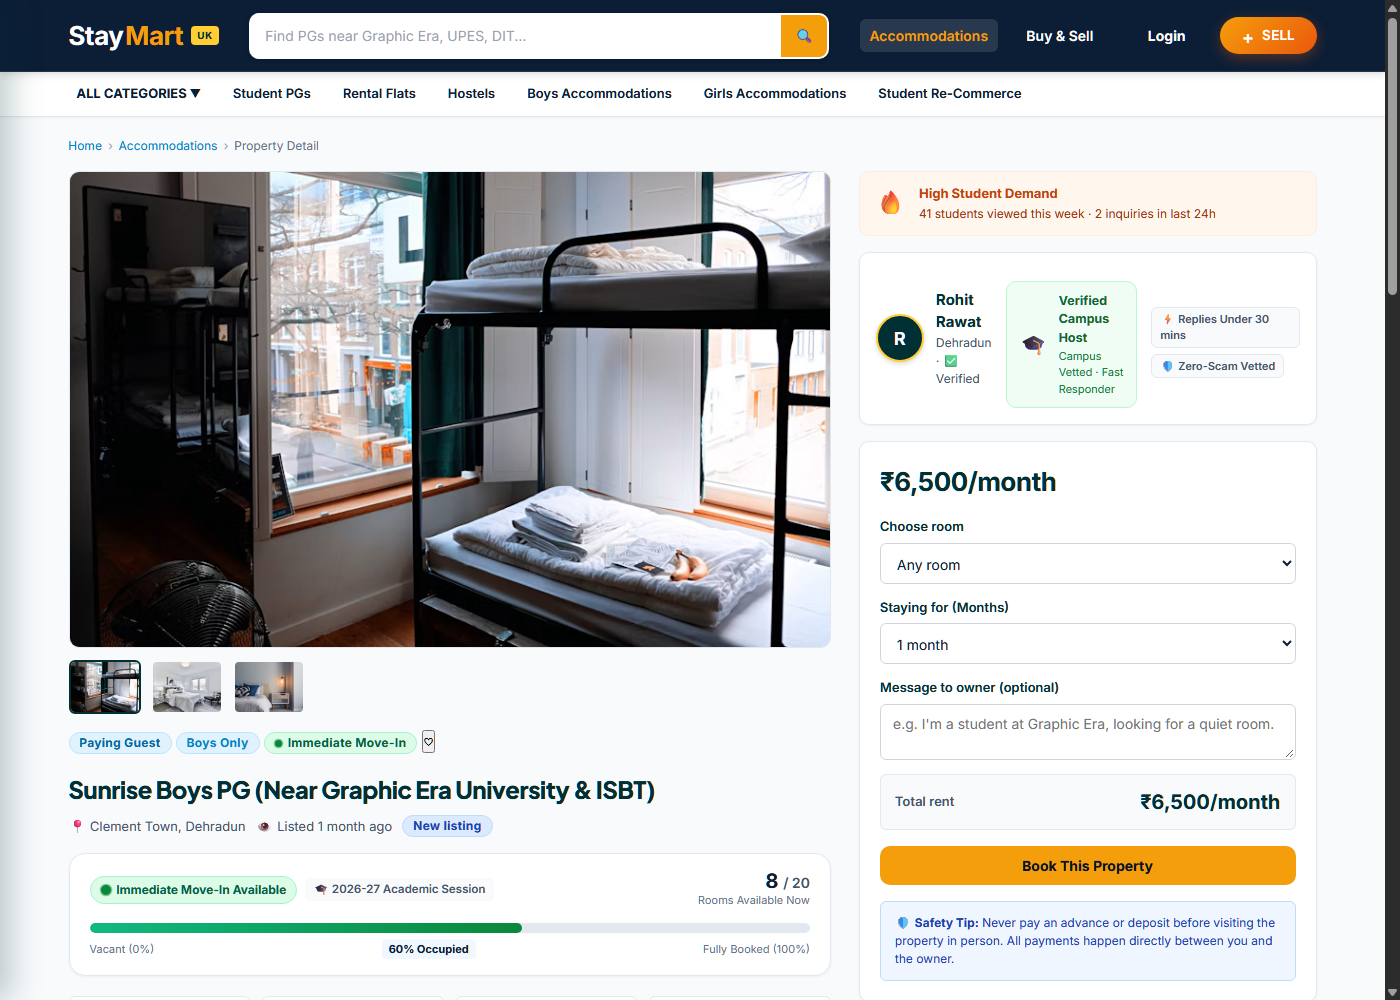
\includegraphics[width=0.92\textwidth]{screenshots/property_detail.png}
    \caption{Step 2: Property Detail View with Room Selection Widget}
    \label{fig:walkthrough_detail}
\end{figure}

\subsection{3. Marketplace Re-Commerce Flow}
Navigating to the Products portal (Figure \ref{fig:walkthrough_product_screens}), students inspect second-hand laptops, smartphones, and furniture listed by graduating seniors.

\begin{figure}[htbp]
    \centering
    \begin{subfigure}[b]{0.48\textwidth}
        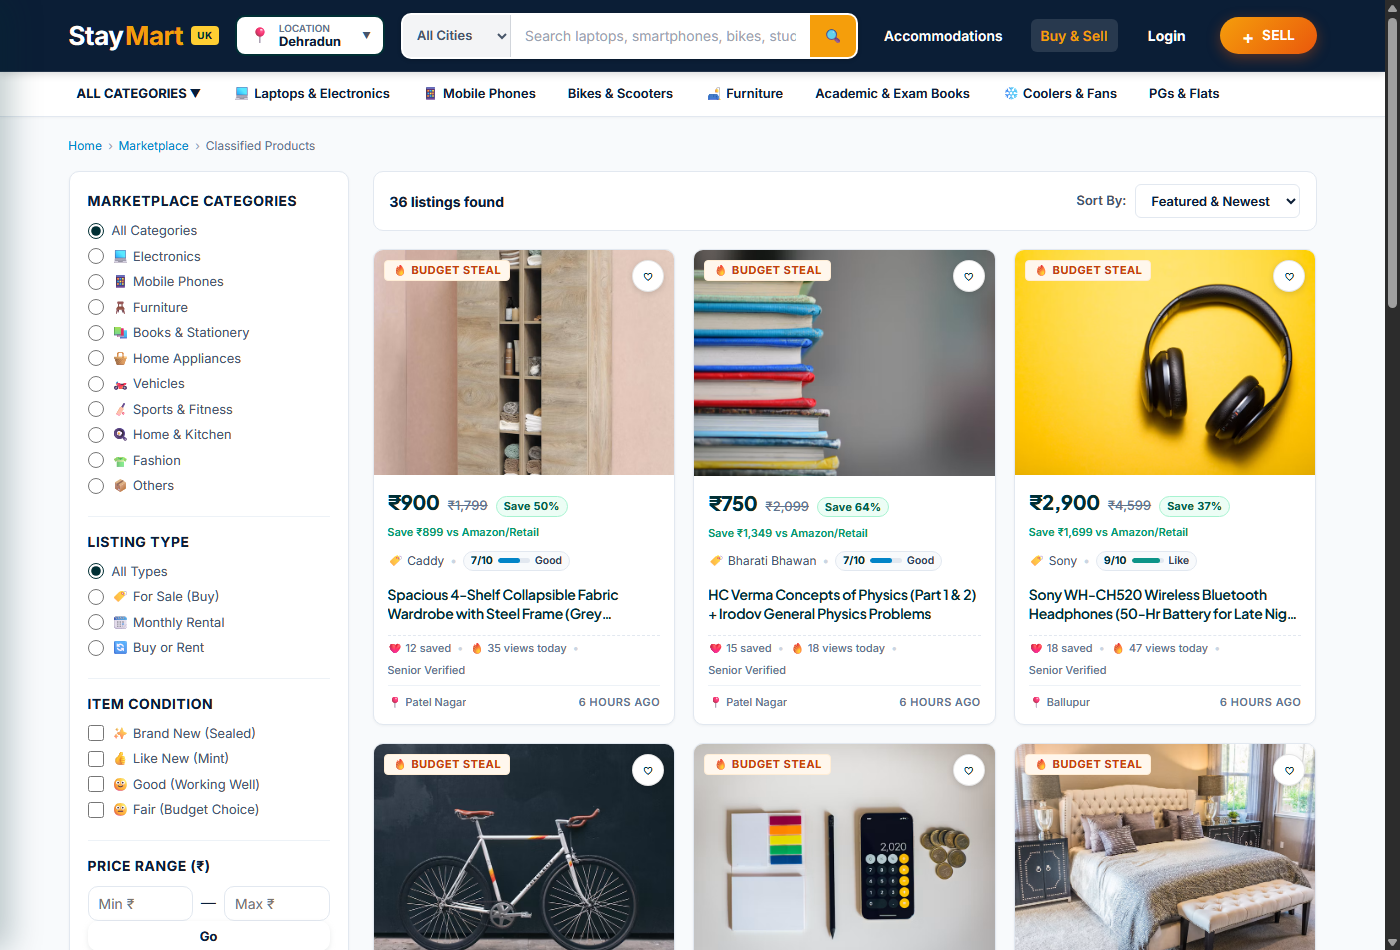
\includegraphics[width=\textwidth]{screenshots/search_products.png}
        \caption{Marketplace Product Catalogue}
    \end{subfigure}
    \hfill
    \begin{subfigure}[b]{0.48\textwidth}
        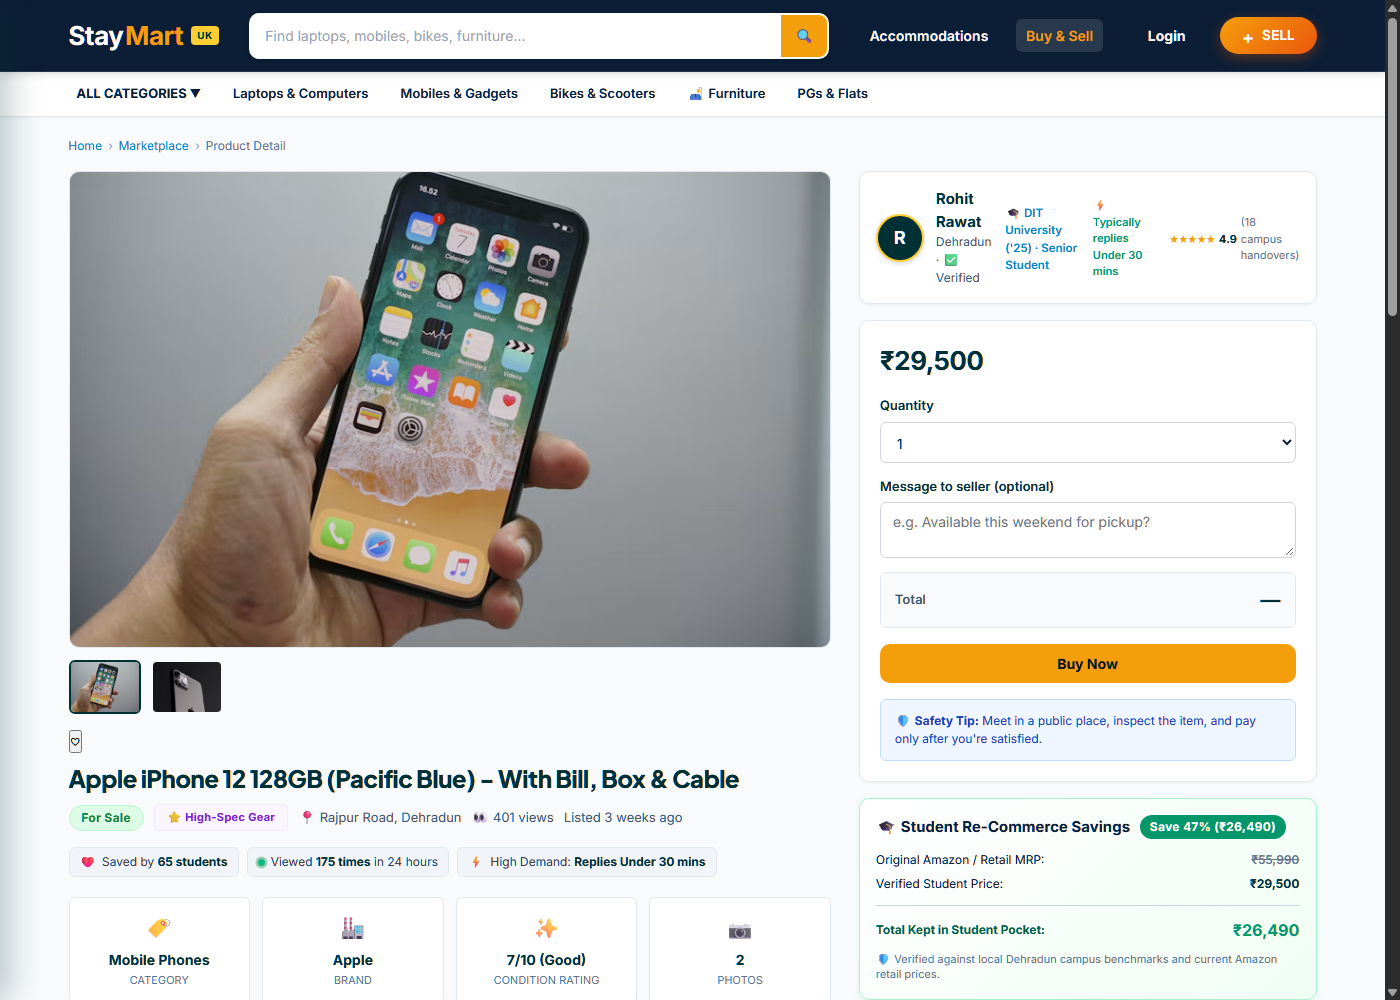
\includegraphics[width=\textwidth]{screenshots/product_detail.png}
        \caption{Product Inspection Page}
    \end{subfigure}
    \caption{Step 3: Marketplace Product Discovery and Inspection}
    \label{fig:walkthrough_product_screens}
\end{figure}

\subsection{4. In-App Conversational Communication}
Clicking ``Message Seller'' initializes a chat session quoting the listing title for context (Figure \ref{fig:walkthrough_chat}).

\begin{figure}[htbp]
    \centering
    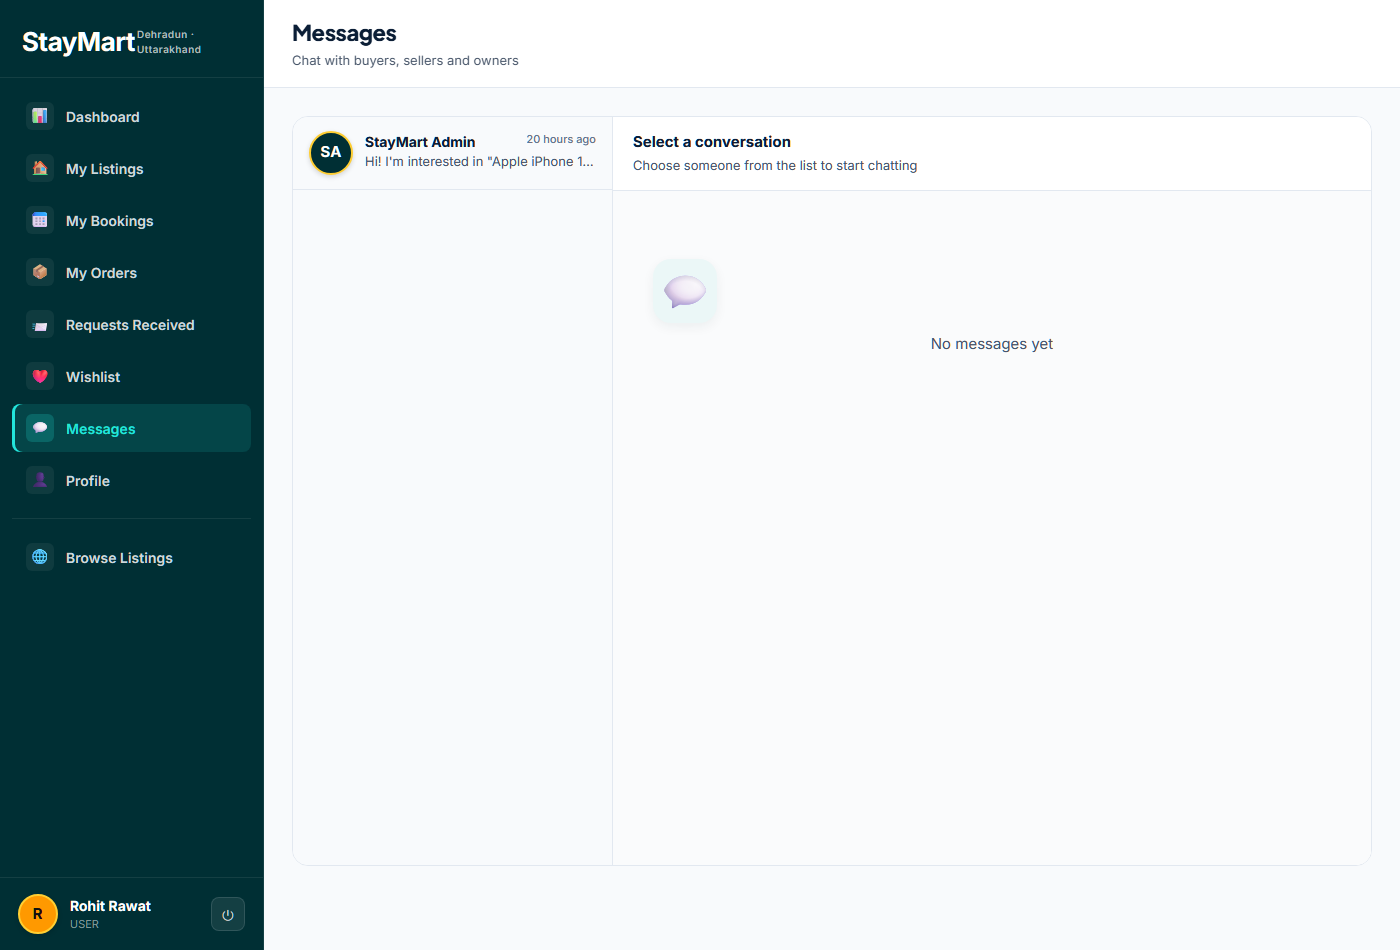
\includegraphics[width=0.92\textwidth]{screenshots/user_chat_active.png}
    \caption{Step 4: Peer-to-Peer Chat Between Student and Caretaker}
    \label{fig:walkthrough_chat}
\end{figure}

\subsection{5. Administrative Moderation and Governance}
Administrators access the moderation dashboard (Figure \ref{fig:walkthrough_admin}) to audit pending submissions and inspect registered student accounts.

\begin{figure}[htbp]
    \centering
    \begin{subfigure}[b]{0.48\textwidth}
        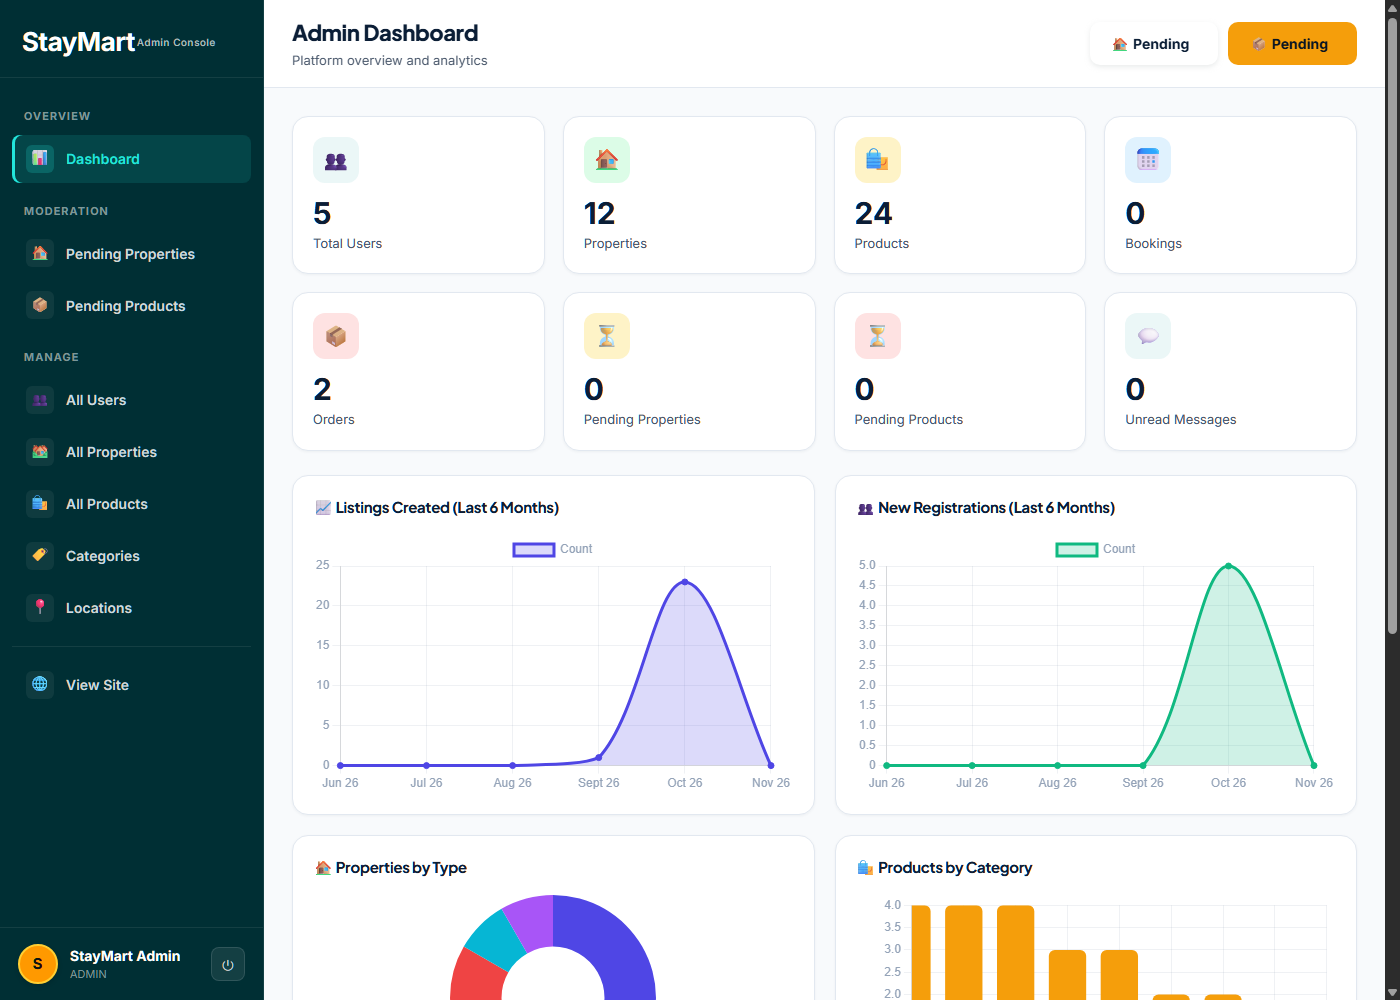
\includegraphics[width=\textwidth]{screenshots/admin_dashboard.png}
        \caption{Administrative Overview and Metrics}
    \end{subfigure}
    \hfill
    \begin{subfigure}[b]{0.48\textwidth}
        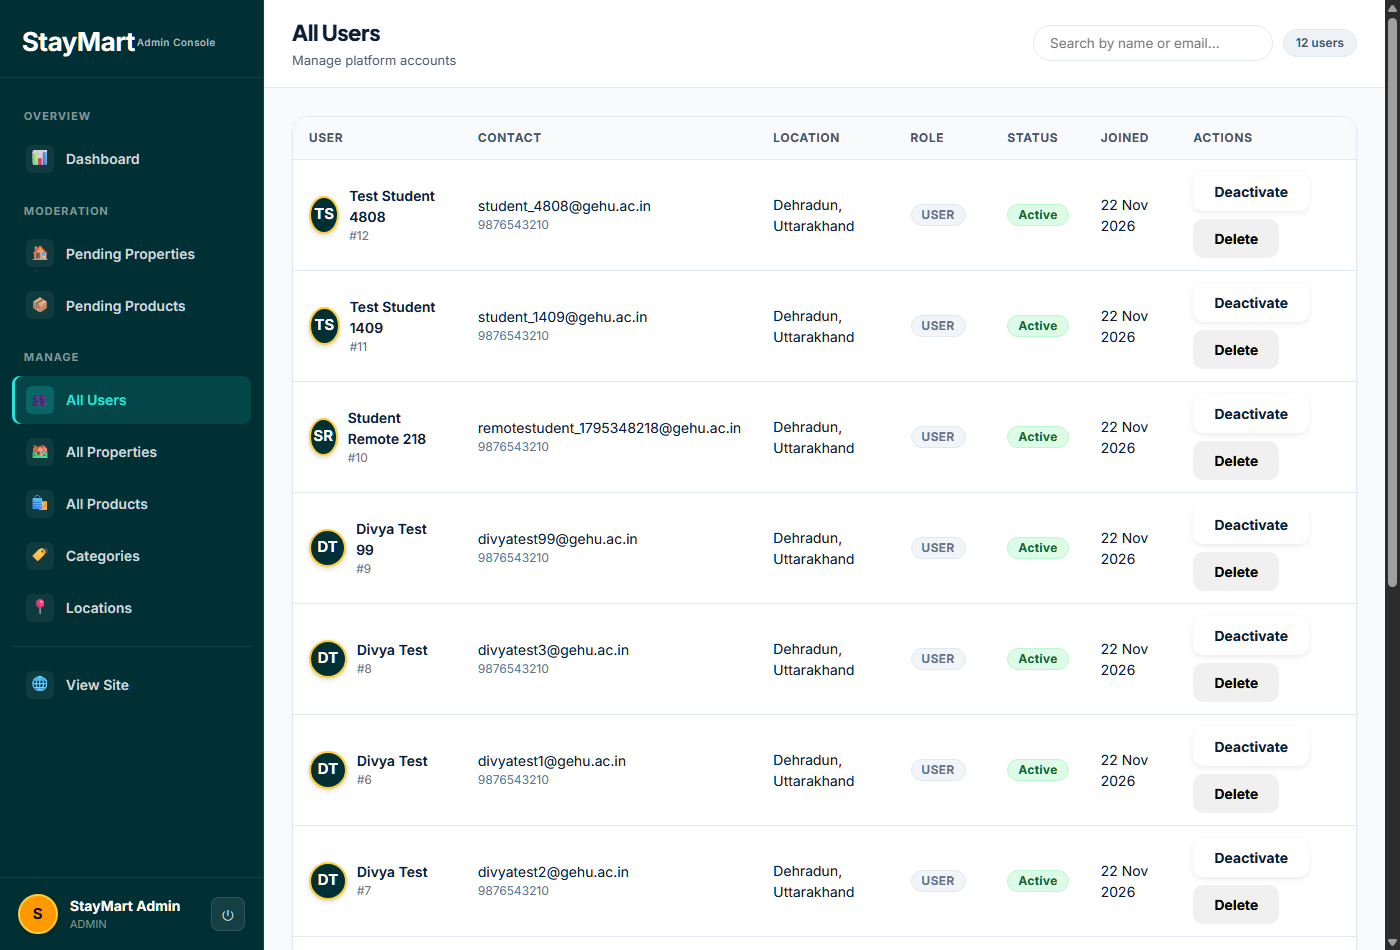
\includegraphics[width=\textwidth]{screenshots/admin_all_users.png}
        \caption{Registered Student Directory}
    \end{subfigure}
    \caption{Step 5: Administrative Dashboard, Moderation Queue, and User Directory}
    \label{fig:walkthrough_admin}
\end{figure}

\subsection{6. User Bookings and Reservation Lifecycle Flow}
Students track reservations and orders in real time (Figure \ref{fig:walkthrough_bookings}). Once confirmed by the host, confirmation vouchers and caretaker contacts are unlocked.

\begin{figure}[htbp]
    \centering
    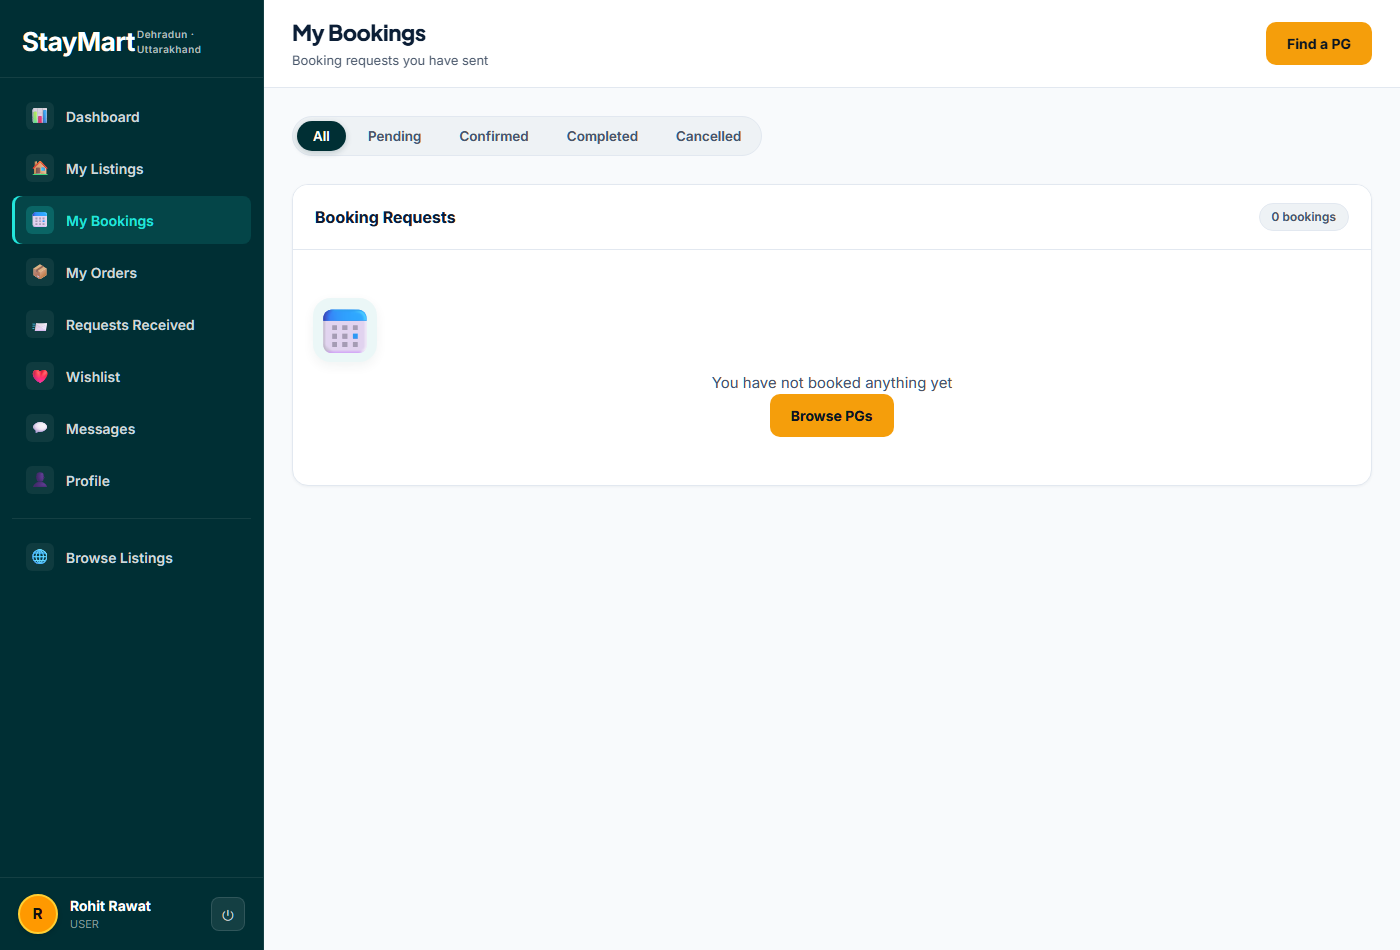
\includegraphics[width=0.92\textwidth]{screenshots/user_bookings.png}
    \caption{Step 6: User Booking Management and Reservation Status Lifecycle}
    \label{fig:walkthrough_bookings}
\end{figure}

\section{Summary}
This chapter verified StayMart across 14 test cases, security penetrations, and 292 automated smoke assertions with zero defects. The visual walkthrough illustrated end-to-end user journeys from search to reservation and admin moderation. The next chapter details cloud deployment and operational procedures.
